%----------------------------------------------------%
%       ANÁLISIS DE LAS TÉCNOLOGÍAS PROPUESTAS       %
%----------------------------------------------------%

\pagestyle{fancy}

\chapter{Análisis de las tecnologías propuestas}
\label{analisis_tecnologias}

\section{Apache Cassandra}

Apache Cassandra es una base de datos distribuida que permite operar sobre grandes volúmenes de datos del tipo clave/valor. Concebida en el 2008 por los ingenieros de Facebook basándose en otros sistemas de almacenamientos distribuidos como Dynamo\cite{decandia2007dynamo} y BigTable \cite{chang2008bigtable}, se caracteriza por ofrecer una  disponibilidad total y mayor escalabilidad lineal en comparación a otras bases de datos NoSQL\cite{nambiartowards}.  Para ello, se basa en un conjunto de nodos homogéneos dentro de una red en anillo que se comunican mediante un protocolo P2P de replicación asíncrona, lo cual permite realizar operaciones de baja latencia para todos los clientes sin necesidad de un servidor maestro.\\

Hoy en día, es utilizada por infinidad de aplicaciones en negocios modernos, siendo la base de datos elegida por un tercio de las compañías que conforman la Fortune 100 \footnote{\url{http://fortune.com/2015/04/14/datastax-hp-sales-partnership/}}. Claro ejemplo de ello son empresas mundialmente conocidas como Apple, Facebook o NetFlix, los cuales utilizan Apache Cassandra como parte de su entramado tecnológico desde hace ya unos años. Cabe destacar que su uso no se limita al mundo empresarial. Muestra de ello es la acogida que ha tenido en el ámbito de la investigación, formando parte en experimentos punteros a nivel mundial como algunos de los realizados en el CERN \cite{sicoe2012persistent}.

\clearpage

\subsection{Funcionamiento}

Las bases de datos NoSQL, en su mayoría, han sido concebidas para resolver un conjunto especifico de problemas. Debido a ello, para entender el funcionamiento de Cassandra cabe resaltar las peculiaridades que la distinguen de los demás sistemas de almacenamiento no relacionales.

\subsubsection{Base de datos distribuida de alta disponibilidad}

El Teorema de Brewer \cite{gilbert2002brewer}, también conocido como Teorema CAP , enuncia que un sistema de cómputo distribuido no puede  garantizar simultáneamente las tres propiedades que se presentan a continuación, solo pudiendo cumplir dos de ellas al mismo tiempo, y acabar cumpliendo la restante tarde o temprano:

\begin{itemize}
	\item \textbf{Consistencia}(Consistency): Todos los nodos ven la misma información al mismo tiempo.
	\item \textbf{Disponibilidad}(Availability): La garantía de que cada petición a un nodo reciba una confirmación de si ha sido o no resuelta satisfactoriamente.
	\item \textbf{Tolerancia al Particionado}(Partition Tolerance): El sistema sigue funcionando a pesar de que haya sido partido por un fallo de red.
\end{itemize}

Para una base de datos distribuida que promete la disponibilidad completa, el Teorema de Brewer implica la incapacidad de garantizar la consistencia total de los datos que almacena y la necesidad de esperar un tiempo indeterminado para que las réplicas de un registro modificado se actualicen correctamente.\\

Para lidiar con dicha restricción, Cassandra ofrece la posibilidad de afinar el nivel de consistencia \footnote{\url{https://docs.datastax.com/en/cassandra/2.1/cassandra/dml/dml_config_consistency_c.html}} en cada consulta, sacrificando para ello parte de la disponibilidad.

\subsubsection{Optimizado para escrituras}

Una de las características a destacar de Cassandra es el elevado ratio de escrituras por segundo que es capaz de realizar, superando notoriamente a otras bases de datos NoSQL en este apartado \cite{rabl2012solving}.\\

Al ejecutar una consulta que desemboca en una escritura, los registros son almacenados en dos estructuras denominadas CommitLog\footnote{\url{https://wiki.apache.org/cassandra/Durability}} y Memtable. El primero, es un fichero donde se adjuntan los registros recibidos, mientras que el segundo, es una cache en memoria que apila dichos registros. Cuando ambas estructuras finalizan de almacenar los datos, Cassandra considera que la consulta ha sido ejecutado satisfactoriamente pudiendo pasar a procesar otras operaciones.\\

Cuando la Memtable\footnote{\url{https://wiki.apache.org/cassandra/MemtableSSTable}} se llena, empieza un proceso de vaciado en el cual primero se dilucida el nodo destinatario de cada registro. Después, dichos registros son escritos de forma secuencial en estructuras inmutables denominadas SSTable, ficheros que representan físicamente el contenido de una tabla. Si esta operación es interrumpida, se utiliza la información almacenada en el CommitLog para recuperar las escrituras perdidas. Finalmente, cuando todos los registros han sido transferidos a su correspondiente SSTable, el CommitLog es purgado.

\begin{figure}[h]
	\centering
	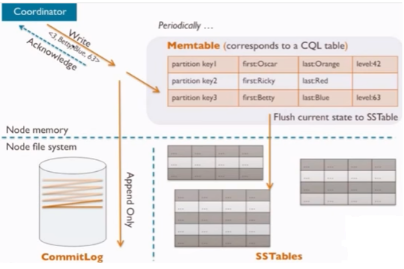
\includegraphics[width=0.65\textwidth]{Ilustraciones/cassandra_data_storage.png}
	\caption{Almacenamiento de datos en Cassandra}
	\label{fig:almacenamiento_cassandra}
\end{figure}

Debido a la naturaleza inmutable de las SSTable, cada vez que la Memtable se vacía un nuevo fichero es generado para representar una tabla ya existente. Ello puede acarrear problemas de eficiencia a la hora de consultar la información de dicha tabla, ya que será totalmente necesario leer todos los ficheros correspondientes. Para sobreponerse a este inconveniente, Cassandra posee un mecanismo llamado compactación que, entre otras acciones, unifica las SSTable que representan una misma tabla eliminando los ficheros restantes. El proceso recién descrito se resume mediante la figura \ref{fig:almacenamiento_cassandra} de la página \pageref{fig:almacenamiento_cassandra}

\subsubsection{Replicación asíncrona sin maestro}

Las bases de datos distribuidas ofrecen la posibilidad de replicar los datos que se almacenan en ellas, lo cual implica que todos los nodos del sistema deban conocer el estado de cada réplica. Cassandra, gracias a un conjunto de mecanismos que se presentan a continuación, es capaz de obtener dicha información de forma local sin depender de un nodo maestro, obteniendo un clúster totalmente homogéneo.\\

\begin{itemize}

\item \textbf{Gossip Protocol}\cite{demers1987epidemic}: Protocolo de comunicación peer-to-peer que intercambia el estado del propio nodo y de aquellos que conoce de forma periódica.

Cada mensaje Gossip tiene una versión asociada a él, gracias al cual el nodo que recibe dicho mensaje puede comparar con la información que posee de antemano y actualizar su conocimiento en caso de ser necesario.
	
\item \textbf{Failure Detector}\cite{chandra1996unreliable}: Conjunto de métodos que mediante mensajes Gossip sugieren de forma local si otro nodo del sistema esta caído o en estado transitorio.

Dentro de la extensa gama de métodos existentes, Cassandra utiliza el Accrual Failure Detector\cite{hayashibara2004spl}. Ofrece la posibilidad de configurar un umbral teniendo en cuenta el rendimiento de red, carga de trabajo, u otras variables. Al cotejar el valor ofrecido por el detector con dicho umbral, Cassandra es capaz de dilucidar si un nodo esta caído, y en caso afirmativo, redireccionar las peticiones a otro activo.

\item \textbf{Merkle Tree}\cite{merkle1987digital}: Árbol hash cuyos nodos padres más altos son, a su vez, hashes de sus respectivos hijos. La ventaja principal es que cada rama del árbol puede ser comprobada de forma independiente, sin la necesidad de descargar todo el conjunto de datos.

La implementación de Anti-Entropia\cite{golay1949notes} en Cassandra, proceso encargado de comparar todas las réplicas de cada dato que existe en el clúster y actualizarlos a la versión más reciente, genera un Merkle Tree por cada tabla durante el proceso de compactación, los cuales se almacenan solo hasta enviarlos a los nodos vecinos. La praxis descrita implica enviar un exceso de datos por la red pero ahorra en operaciones I/O del disco local, lo cual es preferible para conjuntos de datos muy grandes.
	
\end{itemize}

\subsubsection{Sin punto único de fallo}

La ejecución de una consulta es considerada satisfactoria si el clúster es capaz de cumplir con los requisitos de consistencia especificados en la misma. Esta simple premisa se embarulla en un entorno real en donde los nodos de la infraestructura pueden cambiar de estado en cualquier instante y además, seguir cumpliendo con los requisitos de consistencia, dando como resultado el no poder actualizar las réplicas que residen en los nodos temporalmente caídos. 

\begin{itemize}

\item \textbf{Rapid Read Protection}\footnote{\url{http://www.datastax.com/dev/blog/rapid-read-protection-in-cassandra-2-0-2}}: El nodo del clúster que recibe una consulta es denominado coordinador y cumple con el cometido de identificar la máquina menos ocupada entre los que contienen una réplica del registro requerido y redirigir la consulta hacia ella.

Si en ese preciso instante el nodo electo deja de estar disponible, la técnica Rapid Read Protection permite al coordinador escoger otro nodo entre los candidatos y redirigir la petición hacia este último, evitando así tener que devolver un mensaje de error al cliente.

\item \textbf{Hinted Handoff}\footnote{\url{http://www.datastax.com/dev/blog/modern-hinted-handoff}}: Técnica que almacena en una tabla interna del nodo coordinador los registros que no han podido ser replicados a otras máquinas. Al recibir un mensaje Gossip indicando que dichas máquinas vuelven a estar activas, se encarga del envío de los registros correspondientes.

\end{itemize}

\subsection{Cassandra Query Lenguage (CQL)}

El código que rige el funcionamiento interno de las consultas es generado mediante Apache Thrift\cite{slee2007thrift}, una interfaz para implementar llamadas a procedimientos remotos\cite{nelson1981remote} que posibilita el acceso al clúster mediante diversos lenguajes de programación.\\

No obstante, para la gente acostumbrada a trabajar con SQL suponía un escollo familiarizarse con la sintaxis de Thrift. Con el objetivo de atraer usuarios, los desarrolladores de Cassandra optaron por añadir una capa de abstracción para así lograr un lenguaje de consultas que se asemejara sintácticamente a SQL, dando lugar al nacimiento de Cassandra Query Lenguage (CQL).\\

Este lenguaje de consultas presenta las mismas funcionalidades y limitaciones que el antiguo API basado en Thrift, entre las cuales destacan, entre otras muchas, la imposibilidad realizar algunas operaciones como \textit{join}, agrupaciones y agregaciones, además de presentar serias restricciones en la sintaxis de \textit{where}\footnote{\url{https://www.datastax.com/dev/blog/a-deep-look-to-the-cql-where-clause}}

\section{Apache Spark}

Apache Spark\cite{zaharia2010spark} es un proyecto open source de computación en clúster. Desde el principio fue diseñado para ejecutar algoritmos iterativos en memoria sin la necesidad de almacenar en disco los resultados intermedios generados durante el proceso. Esta peculiaridad permite que los procesamientos llevados a cabo con Spark puedan llegar a ser, en algunos casos concretos, 100 veces más rápidos que los de MapReduce\cite{dean2008mapreduce}.\\

La base del proyecto es el denominado Spark Core. Proporciona envío distribuido de tareas, planificación y funciones básicas de entrada salida. La abstracción fundamental de programación se llama Resilient Distributed Datasets\cite{zaharia2012resilient}, una colección lógica de datos particionados a través de las máquinas que se expone mediante una API integrada en lenguajes como Java, Python y Scala.

\subsection{Funcionamiento}

Para el funcionamiento de Spark, es condición sine qua non que los nodos de la infraestructura tengan acceso a la totalidad de los datos que se desea tratar. Ello implica que para procesar un fichero de 25GB, cada nodo tiene que poseer una copia del mismo almacenado en su disco. Esta praxis es inviable, ya que más allá de los problemas de consistencia que generaría, para nada es eficiente ocupar la memoria de todos los nodos con información redundante y procesar el fichero entero cuando en realidad se va a hacer uso de una pequeña porción de dichos datos en cada ejecución.\\

Las bases de datos distribuidas como Cassandra solventan los problemas anteriormente mencionados. Se encargan de distribuir los datos entre diferentes nodos del clúster, ofrecen la posibilidad de acceder a ellos desde cualquier punto y mantienen la consistencia de los mismos a cambio de sufrir una pequeña latencia en el caso de requerir información almacenada en otro nodo de la infraestructura.\\ 

Tal y como se puede apreciar en la figura \ref{fig:spark_initialization} de la página \pageref{fig:spark_initialization}, al ejecutar una aplicación que opera con Spark, un componente denominado \textit{driver} es lanzado. Debido a la necesidad de obtener recursos (CPU y memoria) para llevar a cabo la computación que se le ha encomendado, este se comunica con un nodo del clúster que, mediante especificación previa, adopta el rol de maestro. El \textit{maestro} pregunta a todos los nodos que conforman la infraestructura sobre la cantidad de recursos disponibles que poseen con el objetivo de asignarles los \textit{executors} correspondiente. Las máquinas que alojen al menos un \textit{executor} pasan a denominarse \textit{worker} y a partir de este momento, podrán comunicarse directamente con el \textit{driver} para poder recibir las tareas que éste le envíe.\\

Un \textit{executor} es una unidad de trabajo que se encarga de computar las tareas que le encomienda el \textit{driver}. El número de \textit{executors} que puede albergar cada \textit{worker} está directamente relacionado con el número de recursos que este posee. Spark permite modificar ambos parámetros programáticamente permitiendo así poder amoldarse a las particularidades de cada ejecución.\\

Para transferir el código del programa, residente en la máquina del \textit{driver} en formato JAR, éste adopta  el rol de servidor e intenta enviar el fichero a los \textit{workers}. Si el ejecutable que contiene el código ha sido recibido correctamente por sus destinatarios, estos responden mediante un ACK y en caso contrario, se vuelve a intentar el envío un número determinado de veces. Una vez llegado al máximo de reintentos, el \textit{worker} que no haya enviado el ACK es considerado caído, quedando los \textit{executors} que albergaba fuera del posterior reparto de tareas.

\begin{figure}[h]
	\centering
	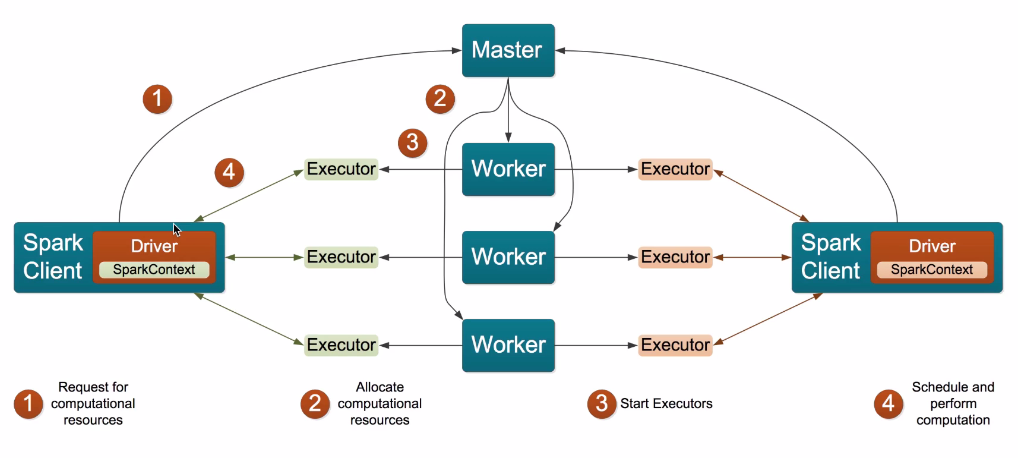
\includegraphics[width=1\textwidth]{Ilustraciones/spark_architecture.png}
	\caption{Arquitectura Spark}
	\label{fig:spark_initialization}
\end{figure}

A la hora de realizar operaciones en Spark, el objeto estrella es el denominado Resilient Distributed Datasets (RDD)\cite{zaharia2012resilient}. Se trata de una abstracción que mediante diferentes APIs disponibles para Java, Scala y Python permite manipular datos distribuidos por los diferentes nodos del clúster como si estuvieran almacenados de forma local. Este objeto es inmutable, lo cual implica que una vez creado no se le pueden añadir nuevos elementos o eliminar los existentes, solo aplicar transformaciones y acciones sobre el.\\

Las operaciones que se pueden realizar sobre las RDD se agrupan, tal y como se ha adelantado antes, en transformaciones y acciones. Las primeras transforman un RDD en otro según el criterio indicado y las segundas realizan modificaciones sobre los datos almacenados en dichas RDD. Cabe destacar que las transformaciones en Spark son operaciones "lazy", lo cual implica que en realidad cada nodo memoriza la secuencia de transformaciones que ha de realizar y los procesa cuando una acción es ejecutada.\\

Una vez terminada la primera fase en la que los \textit{executors} son creados y enlazados con el \textit{driver}, éste último empieza a analizar la estructura del código y genera un grafo DAG (Directed Acyclic Graph)\cite{thulasiraman19925}\cite{bang20082} con las operaciones que se realizan sobre la RDD. Partiendo de ese grafo genera un \textit{job} por cada operación de tipo acción que encuentra y dentro de cada \textit{job} separa la ejecución en diferentes \textit{stages} según las dependencias que existan entre operaciones. Por último, cada \textit{stage} es dividido por defecto en unidades de 64MB y a cada unidad resultante se denomina \textit{task}, el cual es enviado a un \textit{executor} para ser procesado. El tamaño de cada \textit{task} puede ser modificado programáticamente, pudiendo de esa forma manipular el número de \textit{task} que un \textit{executor} deba ejecutar. La figura \ref{fig:spark_task_creation} de la página \pageref{fig:spark_task_creation} ayuda a visualizar la relación entre los elementos que conforman el proceso de creación de tareas.

\begin{figure}[h]
	\centering
	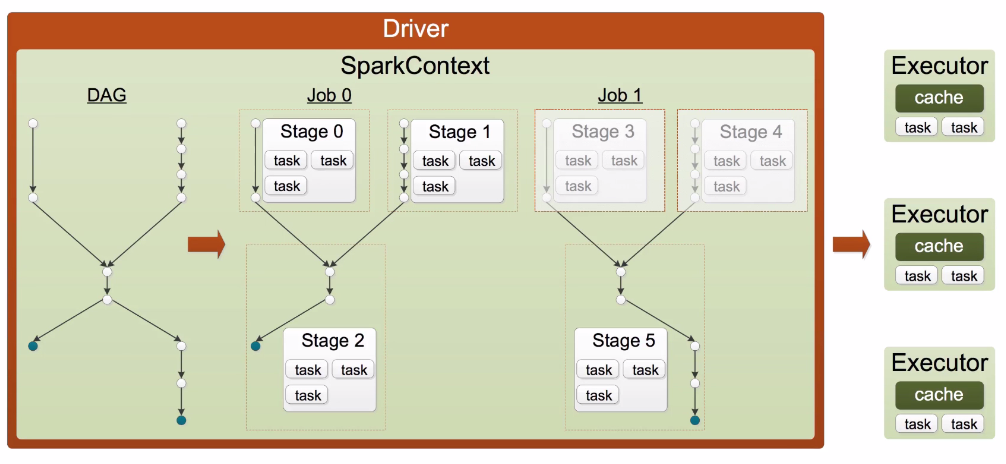
\includegraphics[width=1\textwidth]{Ilustraciones/spark_task_creation.png}
	\caption{Creación de tareas en Spark}
	\label{fig:spark_task_creation}
\end{figure}

El \textit{driver}, una vez habiendo recibido los resultados de todas las \textit{task} que ha repartido, enviará un mensaje a los \textit{executors}
indicando que el procesamiento ha sido finalizado y calculará el resultado final.